\begin{titlepages}
%
\thispagestyle{empty}
\raisebox{0mm}[0mm][0mm]{%
\parbox{8.5in}{
\vspace*{236mm}\hspace{-38.5mm}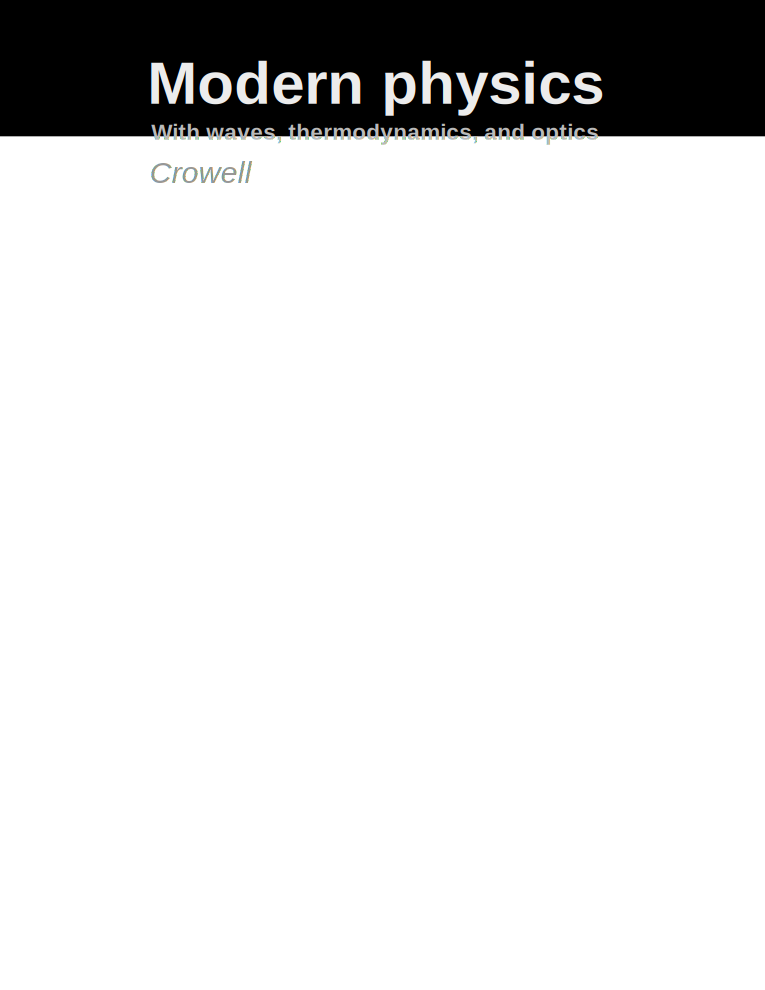
\includegraphics{\chapdir/figs/cover}\\
}
}%
\\


\end{titlepages}

\begin{titlepages}[2]
  \brieftitle
\end{titlepages}

\begin{titlepages}
  \copyrightpage{2019}
  \vspace{100mm}
  \noindent\emph{About the cover:} The cover shows a simulated image of the sky as viewed by an observer who has fallen into a black hole.
  The constellations Orion and Canis Major are visible. Although the observer is already inside the event horizon, the bending
  of light rays by gravity makes it appear as though the black hole only occupies a relatively small part of the field of view.
  The bright ring consists of light from
  stars that are not actually very bright. Their light is amplified because they happen to lie near the event horizon.
  The image was rendered by the open-source library Karl, \url{github.com/bcrowell/karl}. 
  \vfill
\end{titlepages}

\normalsize\normalfont\pagebreak\thispagestyle{empty}\cleardoublepage\thispagestyle{empty}
